\documentclass[aps,prl,reprint]{revtex4-1}
\usepackage{blindtext}

\usepackage{amsmath}
\usepackage{graphicx}

\begin{document}
\title{Fabry Perot Interferometer}
\author{Xueqi Li}
\noaffiliation
% \date{Feb 4, 2017}
% \email{xueqi.li@stonybrook.edu}

% \begin{abstract}
% Here I tell what I have done... And I have done a lot but it is hard to tell what exactly I have done...
% \end{abstract}

\maketitle

\section{Introduction}  
The idea of the Fabry-Perot interferometer is that to multiple reflect a single light between two mirrors.

The outcoming light will have phase as following:
\[
2 \pi \frac{(2n-1) L \cos\theta}{\lambda}
\]
Thus, we have electric field that be transmitted as following:
\[
E_T = \frac{E_0 t^2}{1-r^2e^{i\delta}}
\]
there $t$ and $r$ are transmittance and reflectance. Thus, we have light intensity proportional to $|E_T|^2$. Which give us following equation:
\[
I_T = I_0 \frac{T^2}{|1-Re^{i\Delta}|}
\]
where $T = tt^*$, $R = rr^*$, $\Delta = \delta + \delta_r$. And we can have following equation:
\[
I_T = I_0 \frac{T^2}{(1-R)^2}\frac{1}{1+\mathcal{F}\sin^2(\frac{\Delta}{2})}
\]
where $\mathcal{F} = \frac{4R}{(1-R)^2}$.

In the lab, we will try to measure the full width at half max. Let say we have max intensity at $\Delta_0$, using the small angle approximation, we can find $\Delta_0 = \frac{2}{\sqrt{\mathcal{F}}}$. From above result we can see that full width at half max is $\frac{4}{\sqrt{\mathcal{F}}}$.


\section{Part I}
\subsection{Procedure}
\begin{enumerate}
    \item Set up the interferometer and the light source. A small aperture will be used between the interferometer and the photometer.
    \item Adjust the movable mirror of the interferometer so that the interference image clearly shows on the screen between the interferometer and the photometer.
    \item remove the screen. Move the photometer to the center of the interference image.
    \item Recored the reading of the photometer, and move the photometer left a step distance.
    \item redeo last step untill we have enough data.
    \item Analyze data and error.
\end{enumerate}
\subsection{Data}
The distance between the interferometer and the photometer ($l$) is 75$\pm$2cm
Please find the data table in appendix.
\subsection{Analysis}
First we need to convers to angle. Knowing the distance between the interferometer and the photometer, the angle is given by $\theta = \tan^{-1} \frac{d}{l}$, where the error is 
\[
\sqrt{(\frac{l \sigma_d}{d^2+l^2})^2 + (\frac{d\sigma_l}{l^2+x^2})^2}
\]
After that we can use the pahse euqaiton to convers this angle to $\Delta$. Thus, we can have following plot:
\begin{center}
 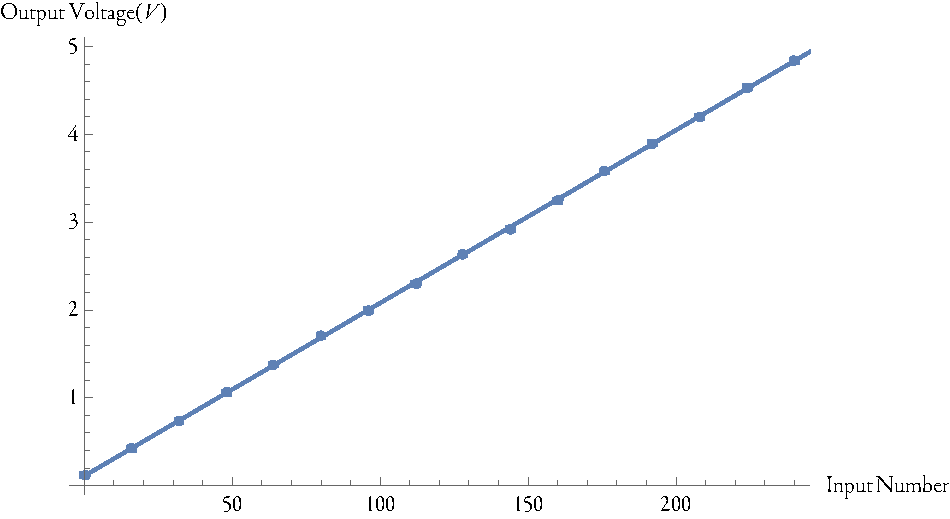
\includegraphics[height=1.8in]{plot.pdf}
\end{center}
We can kind of identify the first peak at 4-th, 5-th, and 6-th datapoint, and we can have the value of the full width at half max is about $6.874\pm5.175$.

\section{Part II}
\subsection{Procedure}
\begin{enumerate}
    \item Remove the moveable mirror of the interferometer.
    \item Recored the reading of the photometer.
    \item Completely remove the interferometer (another mirror) without changing the distance between the light source and the photometer.
    \item Recored the data.
    \item Analyze data and error.
\end{enumerate}
\subsection{Data}
\[
I_{\mathrm{with}} = 14.3 \pm 0.2, I_\mathrm{without} = 15.7 \pm 0.2
\]
\subsection{Analysis}
We can compute that $r = \frac{I_\mathrm{without} - I_{\mathrm{with}}}{I_\mathrm{without}} = \frac{15.7 - 14.3}{15.7} = 0.089$, where the error is 
\[
\sqrt{\sum_{\mathrm{with, without}}(\frac{\partial}{\partial I_i} \frac{I_\mathrm{without} - I_{\mathrm{with}}}{I_\mathrm{without}})^2\sigma_{I_i}^2} 
\]
that is
\[
\sqrt{ \left(\frac{\sigma_{I_\mathrm{without}} I_\mathrm{with}}{I_\mathrm{without}^2}\right)^2 + \left(\frac{\sigma_{I_\mathrm{with}} }{I_\mathrm{without}}\right)^2}
\]
and we can compute it as 0.017.

Thus we can compute that $\mathcal{F} = \frac{4R}{(1-R)^2} = 0.4290$, where $R = rr^*$. For the error, it is 
\[
\sigma_\mathcal{F} = \frac{\partial}{\partial R} \frac{4R}{(1-R)^2} \sigma_R = \frac{4(R+1)}{(R-1)^3}\sigma_R  = 0.0892
\]

To compare with the result of part I, $\frac{4}{\sqrt{\mathcal{F}}} = 6.107\pm0.635$


\section{Conclusion}
The reust is not good. The data in the first part is too fuzzy. The reason for taht is we have a larger $r$. To improve it, we need a better interferometer with a higher $r$. Also, the erorr on Intensity is 






%\begin{center}
% 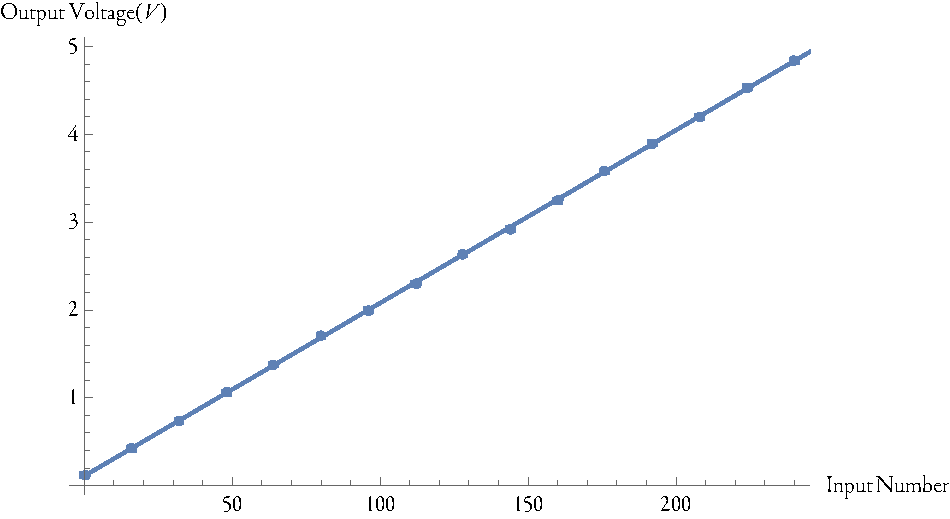
\includegraphics[height=1.3in]{plot.pdf}
%\end{center}

% \blindtext \cite{article-minimal}

% \bibliographystyle{apsrev4-1} % Tell bibtex which bibliography style to use
% \bibliography{xampl} % Tell bibtex which .bib file to use (this one is some example file in TexLive's file tree)

\end{document}